\cotefile{31}
\scanpage{52}
% archive sheet number: 51

% L1–4, upper lemma
\uline{Lemme 2} Soit $k$ un corps, tel que $H^i(k',\Gamma)=0$ pour $\unsure{i|l}>n$. \inserted{et tout groupe abélien fini $\Gamma$ où $\unsure{G'_k|G_{k'}}$ opère trivialement, et tte extension finie $k'$ de $k$.} Soit $K$ une extension de \deleted{\unsure{$k$}} type fini de $k$, de degré de transcendance $1$. Alors $H^i(K,\Gamma)=0$ pour $i>n+1$.

% L5–7, left field diagram
\diagram{\begin{tikzcd}[ampersand replacement=\&,column sep=small,row sep=small]
k \arrow[d,dash] \& \&\\
k'=\widetilde{k}\cap K \arrow[d,dash] \& K \arrow[l,dash] \arrow[d,"G''"'] \arrow[dr,"G"] \&\\
\widetilde{k} \arrow[r,dash] \& \widetilde{k}K \arrow[r,"G'"'] \& \widetilde{K}\deleted{K}
\end{tikzcd}}

% L5–7, right of diagram
\unsure{Cons.|On a|d'où} \unsure{sa|la|une} suite exacte

% L6–7, exact sequence
\[
e \mathbin{\unsure{-|\to}} G' - G - G'' - e,
\]

% L8–12, spectral sequence and vanishing
d'où une suite spectrale $\underline{H}^i(G'',\underline{H}^j(G',\Gamma))\Longrightarrow\underline{H}^{\unsure{*|\times}}(G,\Gamma)$. Or $H^j(G',\Gamma)=0$ si $j>1$ en vertu du lemme 1, et d'autre part, \deleted{$G''$ étant un sous-groupe d'indice fini de} \inserted{$\underline{H}^i(G'',\underline{H}^j(G',\Gamma))=0$ si $i>n$, par} l'hypothèse. D'où par suite $H^p(G,\Gamma)=0$ si $p>n+1$, cqfd.

% L13–16, corollary
\uline{Corollaire} Soit $K$ un corps de fonctions algébriques sur un corps algt. clos $k$, $\mathrm{deg.tr.}_k K=n$. Alors $H^i(K,\Gamma)=0$ pour $i>n$ et tout groupe \inserted{abélien} fini $\Gamma$ où $G_K$ opère trivialement.
\scanpage{54}
% archive sheet number: 53

% L1, upper right
\deleted{\uline{\unsure{Notes et conjectures}}}

% L2–5, title
Th. fondamental des morphismes propres. [Cohomologie \unsure{discrète|discriti|de base}\,\ldots] : \uline{Théorème d'échange}

% L6, below title
Questions marginales

% Upper centre, pencil
\margin{\unsure{6 p|6 p.}}
\scanpage{55}
% archive sheet number: 54

% L1–5, question
\uline{Question} $X$ espace topologique, $Y$ fermé de $X$, $F$ faisceau \uline{injectif} sur $X$, est-il vrai que $H^i(Y,F|Y)=0$ pour $i>0$ [d'où résulterait que $H^i(V,F|V)=0$ pour tt ouvert $V$ de $Y$, $i>0$]. Réponse \uline{négative}.

% L6–7, after answer
Tout d'abord, il n'est pas vrai que pour un faisceau $F$ sur $X$, \unsure{$=$|même} injectif, l'hom \unsure{(injectif)|(surjectif)}

% L8, restriction
\[
\underset{\substack{U\ \mathrm{vois.}\\ \mathrm{de}\ Y}}{\underrightarrow{\lim}}\ \deleted{\unsure{H}}\ H^0(U,F)\longrightarrow H^0(Y,F)
\]

% L9–11, continuation
soit aussi \uline{surjectif}, i.e. qu'une section se prolonge à un voisinage [i.e. à $X$ tt entier si $F$ est flasque, p.ex. injectif]

% L12–19, first example
\uline{Ex 1} $X$ espace irréductible, $Y$ formé de deux pts fermés distincts \inserted{$a,b$}, $F$ faisceau des applications \unsure{quelc.} dans $\mathbb{Q}$, la section de $F|Y$ qui est le germe $0$ en $a$, le germe $1$ en $b$, ne se prolonge ``pas'' \deleted{\unsure{[à la}} à \deleted{un voisinage} $X$, car si oui la section prolongée serait $0$ sur un voisinage $U$ de $a$, $1$ sur un voisinage $V$ de $b$, or $U\cap V\ne\varnothing$, absurde.

% Left of L14–16, two points
\figure{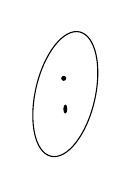
\begin{tikzpicture}[x=1cm,y=1cm]\draw[thin,rotate=-13] (0,0) ellipse (.38 and .81);\fill (-.02,.20) circle (.032); \fill (.00,-.19) ellipse (.025 and .057);\end{tikzpicture}}

% L20, between examples
Ici, $X$ \unsure{pourrait|pouvant} être variété algébrique.

% L21–23, second example
\uline{Ex 2} \unsure{\={M}} exemple \inserted{essentiellement} que le précédent, mais $Y$ étant irréductible, par exemple une droite dans le plan (\unsure{topologie|topologies} de Zariski).

% Left of L22–23, secant
\figure{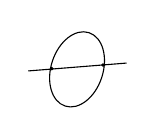
\begin{tikzpicture}[x=1cm,y=1cm]\draw[rotate=-18] (0,0) ellipse (.33 and .49);\draw (-.62,-.02)--(.63,.08);\fill (-.32,.01) circle (.025);\fill (.33,.055) circle (.025);\end{tikzpicture}}
\scanpage{56}
% archive sheet number: 55

% Top left, loose mark
\margin{$X$}

% L1–4, upper left
\figure{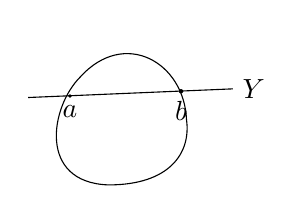
\begin{tikzpicture}[x=1cm,y=1cm]\draw (0,-.55) .. controls (-.90,-.52) and (-.74,.44) .. (-.36,.82) .. controls (.20,1.44) and (.96,1.01) .. (.99,.28) .. controls (1.05,-.15) and (.77,-.55) .. (0,-.55);\draw (-1.02,.56)--(1.58,.67) node[right] {$Y$};\fill (-.49,.58) circle (.024) node[below] {$a$};\fill (.92,.64) circle (.028) node[below] {$b$};\end{tikzpicture}}

% L1–8, following Ex 2
Considérons $X_1={}$ cercle cf figure, et le faisceau $F_1$ \inserted{sur $X_1$} des applications dans $\mathbb{Q}$, soit $F$ son image sur $X$. La question de prolonger une section sur $Y$ à $X$ est équivalente à celle de prolonger une section sur $Y\cap X_1$ à $X_1$, \uline{or on a} vu que c'est en général impossible.

% L9–12, third example
\uline{Ex 3} Un faisceau induit par un injectif n'est généralement pas flasque \inserted{(ni mou)} ; les \inserted{Exemples 1 et 2 prouvent qu'un faisceau \deleted{flasque} \inserted{injectif donc flasque} n'est pas néc. mou, donc il \unsure{n'y a qu'à prendre|n'y a qu'à faire} $X=Y$]} \deleted{de façon précise, dans le cas de l'ex 2, le faisceau $F|Y$}

% L13–15, cancelled paragraph
\deleted{Soient $X,Y$ comme dans l'exemple 2, $F$ étant cette fois ci le faisceau des applications de $X$ dans $\mathbb{Q}$,}

% L16–20, lower right
On ne s'en tire pas \unsure{sur|pour} $Y$ une courbe \uline{irréductible} [\unsure{ici|car|i.e.}, \unsure{ds ce cas} le faisceau induit est tjrs flasque, facile].

% L16–19, lower left
\figure{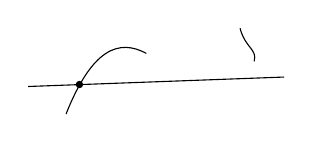
\begin{tikzpicture}[x=1cm,y=1cm]\draw (0,0)--(3.25,.12);\draw (.48,-.35) .. controls (.81,.48) and (1.15,.61) .. (1.50,.42);\fill (.65,.025) circle (.047);\draw[thin] (2.69,.74) .. controls (2.76,.48) and (2.91,.48) .. (2.87,.32);\end{tikzpicture}}

% L21–23, foot
Mais prenons pour $Y$ la réunion de 2 courbes \inserted{$Y_1$ et $Y_2$ \deleted{\unsure{ds}}} se coupant en $\unsure{0|a}$, dans $X$ \inserted{\uline{irréd}}
\scanpage{57}
% archive sheet number: 56

% L1–4, upper left
\figure{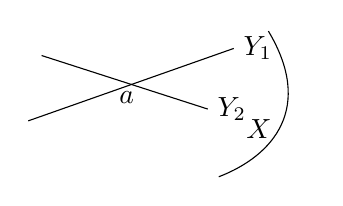
\begin{tikzpicture}[x=1cm,y=1cm]\draw (-1.25,-.47)--(1.36,.45) node[right] {$Y_1$};\draw (-1.08,.36)--(1.03,-.32) node[right] {$Y_2$};\node[below] at (0,.02) {$a$};\draw (1.80,.67) .. controls (2.38,-.30) and (1.87,-.91) .. (1.17,-1.18);\node at (1.68,-.58) {$X$};\end{tikzpicture}}

% L1–12, extending the section
Soit $F$ le faisceau \inserted{sur \deleted{\unsure{$X$}}} des applications \unsure{quelc.} dans $\mathbb{Q}$, et $Y'=Y-\{a\}$, considérons la section de $F|Y'$ qui est $0$ sur $Y'_1$, $1$ sur $Y'_2$, on ne peut la prolonger à $Y$, car \unsure{si on|si l'on} pouvait, il y aurait un voisinage ouvert $U$ de $a$, et une application $U\longrightarrow\mathbb{Q}$ qui \deleted{\unsure{en les pts de} $Y'_1$ ($Y'_2$) \unsure{serait}} au voisinage de $Y'_1$ ($Y'_2$) induirait $0$ ($1$), absurde car ces voisinages doivent se couper !

% L13–17, cancelled development
\deleted{On ne peut cependant s'en tirer avec $Y$ une \uline{courbe} pour \unsure{contre-exempler} le pb du début. En \unsure{effet}, décomposant $Y$ en ses composantes \inserted{irr.} $Y_i$, on aurait un}

% L17, cancelled sequence
\[
\deleted{F_{\deleted{\unsure{Y}}Y}\longrightarrow\prod_i F_{Y_i}\longrightarrow G\longrightarrow0},
\]

% L18–19, cancelled continuation
\deleted{$G$ concentré en un ens fini, d'où \deleted{$H^{\unsure{1|0}}$} (les $F_{Y_i}$ étant flasques, d'où $H^1(Y,F_{Y_i})=0$]}

% L20, cancelled cohomology sequence
\[
\deleted{\deleted{\unsure{H^1(}}\quad\prod_i H^0(\unsure{X|Y|Y_2},F_{Y_i})\longrightarrow \deleted{\unsure{G}}H^0(Y,G)\longrightarrow H^1(Y,F_Y)\longrightarrow 0}
\]
\scanpage{58}
% archive sheet number: 57

% L1–8, example 4
\uline{Exemple 4} \unsure{Donnons|Donnant} un contre-exemple à la question du début. $Y$ est formé de deux courbes irréductibles \inserted{$Y_1,Y_2$} se coupant en 2 pts $a,b$, dans $X$ irréductible. $F$ est le faisceau des applications de $X$ dans $\mathbb{Q}$. \deleted{On a} \unsure{Cons.|On a} la suite exacte

% L4–8, upper left
\figure{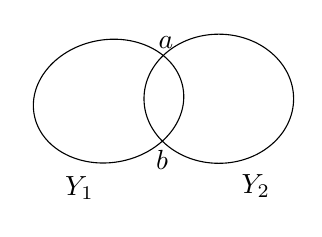
\begin{tikzpicture}[x=1cm,y=1cm]\draw[rotate=10] (0,0) ellipse (.96 and .78);\draw (1.40,.03) ellipse (.95 and .82);\node[above] at (.73,.54) {$a$};\node[below] at (.68,-.50) {$b$};\node[below] at (-.37,-.83) {$Y_1$};\node[below] at (1.87,-.81) {$Y_2$};\end{tikzpicture}}

% L9, cohomology sequence
\[
H^0(Y_1,F_1)\times H^0(Y_2,F_{Y_2})\longrightarrow
\underset{\substack{\deleted{\unsure{H}}\ \shortparallel\\F_a\times F_b}}{H^0(Y_{12},\deleted{\unsure{F_{Y_{12}}}} F_{12})}
\mathbin{\unsure{-|\to}}H^1(Y,F_Y)\longrightarrow0
\]

% L10–15, explanation
[$F_i=F_{Y_i},\ \unsure{F_{12}|H_{12}}=F_{Y_{12}}$] donc la question est de représenter un élément de $H^0(Y_{12},F_{12})=F_a\times F_b$ comme \uline{différence} $f_1-f_2$, où $f_i\in H^0(Y_i,F_i)$. \unsure{Je prend|On prend} l'élmt $(0,1)\in F_a\times F_b$, je dis qu'il ne se représente pas comme diff.

% L16–22, proof and overwritten line
En effet, si on avait une solution $f_1,f_2$, on aurait un voisinage $U$ \inserted{($U'$)} de $a$ \inserted{($b$)}, et \deleted{\unsure{$\varphi,\varphi'$}} tel \deleted{\unsure{que,} \unsure{$\varphi$}} $\unsure{\varphi|\phi}_1,\varphi_2\in\Gamma(U,F)$ \deleted{\unsure{\,$\varphi,\varphi'\in\Gamma(U,F)$}} [$\varphi'_1,\varphi'_2\in\Gamma(U,F)$] \deleted{\unsure{$\varphi',\varphi'\in\Gamma$}} tels que pour tt $x\in Y_i\cap U$, on ait $f_{ix}=\varphi_{ix}$ ($x\in Y_i\cap U'$ on ait $f_{ix}=\varphi'_{ix}$). De plus, prenant $U$ ($U'$) assez petits, on devra avoir \deleted{\unsure{$f$}} $\varphi_2\unsure{-|=}\varphi_1=0$ [resp. $\varphi'_2-\varphi'_1=1$] ;

% L22–26, heavily crossed lower continuation
\deleted{alors, prenant \unsure{de un} alors un fermé de $X$ ne contenant pas \unsure{qui} tt pt de $x\in Y_1\cap U\cap U'$ \unsure{assez} au \unsure{autre} $a$ ni $b$ [réunion d'un voisinage de $Y_1$ et d'un voisinage de $Y_2$] on devra avoir} On aura alors $\varphi_{1x}=\varphi'_{\unsure{1|2}x}$ \deleted{$(=f_{1x})$, \unsure{et voir}} pour $x\in$
\scanpage{59}
% archive sheet number: 58

% L1–6, overlap of neighbourhoods
$x\in U\cap U'\cap Y_1$ \deleted{donc} dans un voisinage $W_1$ de $U\cap U'\cap Y_1$, et $\unsure{\varphi|\phi}_{2\deleted{\unsure{1}}x}=\varphi'_{2x}\,(=f_{2x})$ \deleted{pour $x$ dans i.e. $\varphi_{1x}=\varphi$} pour $x\in U\cap U'\cap Y_2$, donc $\varphi_{1x}=\varphi'_{1x}+1$ pour $x\in U\cap U'\cap Y_2$, donc pour $x$ dans un voisinage $W_2$ de $U\cap U'\cap Y_{2}$. Donc si $x\in W_1\cap W_2$, on aura \deleted{\unsure{al.}} à la fois

% L7, two equalities
\[
\varphi_{1x}=\varphi'_{2x}\qquad\text{et}\qquad\varphi_{1x}=\varphi'_{1x}+1
\]

% L8–9, contradiction
i.e. $0=1$, absurde [compte tenu que $W_1\cap W_2\ne\varnothing$, $X$ étant irréductible].

% L10–11, below rule
Utilisant cet exemple, on trouve un exemple avec $Y$ \uline{irréd} (de \uline{dim 2} \inserted{ds $X$ de dim 3}],

% L12–16, new construction
Pour ceci, dans $X$ on \unsure{considère|considèrera|considérant} un $X_1$ \inserted{fermé (dim 2)} qui recoupe $Y$ suivant la figure $Y_1=X_1\cap Y$ précédente

% L13–15, left plane
\figure{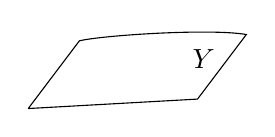
\begin{tikzpicture}[x=1cm,y=1cm]\draw (0,0)--(2.15,.12)--(2.77,.94) .. controls (2.31,1.02) and (.94,.93) .. (.65,.86)--(0,0);\node at (2.23,.63) {$Y$};\end{tikzpicture}}

% L16, inline pair of curves
\figure{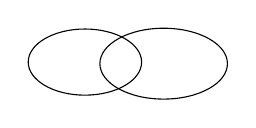
\begin{tikzpicture}[x=1cm,y=1cm]\draw (0,0) ellipse (.72 and .42);\draw (1.00,-.02) ellipse (.81 and .45);\end{tikzpicture}}

% L16–18, foot
. On prend alors le faisceau $F$ sur $X$ extension \unsure{can|can.} du faisceau des applications de $X_1$ dans $\mathbb{Q}$.
\scanpage{60}
% archive sheet number: 59

% L1–3, proposition
\uline{Proposition} $F$ faisceau abélien sur un espace top. (ordinaire) $X$. Conditions équivalentes

% L4, condition i
(i) Pour tt ouvert $U$ de $X$, $H^1(U,F)=0$

% L5, condition i bis
(\deleted{\unsure{ii}}\unsure{i bis|ii}) Pour tt ouvert $U$ de $X$, $H^i(U,F)=0$ pour $i>0$.

% L6, condition ii
(\deleted{\unsure{iii}}\unsure{ii|iii}) \inserted{[pour $X$ noeth]} Pour deux ouverts $U,V$ de $F$,

% L7, two-open formula
\[
H^1((U,V);F)=H^0(U\cap V,F)/\operatorname{Im}\big(H^0(U,F)\times H^0(V,F)\big)
\]

% L8, continuation
est nul.

% L9–10, condition ii bis
(ii bis) Pour tt ouvert $U$ et tt recouvrement \inserted{ouvert} $\underline{U}=(U_i)$ de $U$, on a

% L11, cover cohomology
\[
H^i(\underline{U},F)=0\qquad\text{pour}\quad i>0.
\]

% L12–14, first equivalence
(i bis) $\Longrightarrow$ (ii bis) par suite spectrale de Leray, est bien connu (petit argument de Cartan en une direction)

% L15–16, two implications
\[
\begin{aligned}
(\mathrm{i\ bis})&\Longrightarrow(\mathrm{i})\\[-2pt]
(\mathrm{ii\ bis})&\Longrightarrow(\mathrm{ii})
\end{aligned}
\quad\text{trivial}
\]

% L17–21, final argument
(i) $\Longleftrightarrow$ (ii) En effet $H^1(\deleted{\unsure{\{} }U\cap V,F)\subset H^1(U\cup V,F)$, d'où (i) $\Rightarrow$ (ii), pour (ii) $\Longrightarrow$ (i) on \deleted{\unsure{prend}} considère $\unsure{\zeta|\xi}\in H^1(U,F)$, \deleted{\unsure{on note}} considère un ouvert $U'\subset U$ \uline{maximal} \inserted{(N.B. $X$ noeth)} où $\zeta$ soit nul, je dis que $U'=U$, \unsure{on regarde un|en regardant}.
\scanpage{61}
% archive sheet number: 60

% L1–6, NB
\uline{NB} $l-k-K$ donnés, pour que, pour \uline{tte} extension $L$ de t.f. (ou finie) de $K$, on ait \deleted{$N_{L/K}$} $\delta(L/K,k/l)=0$ i.e. $k$ soit $l$-\unsure{admissible} pour $L/K$ il faut \uline{\unsure{s.} que} $k\subset l(K^p)$ \inserted{i.e. $k(K^p)\subset l(K^p)$}

% L7, middle left
Car si $\underline{K-L=K(x)}$

% L7, middle right
\[
x^p\in k,\quad x^p\notin l(K^p)
\]

% L8, on brace
\unsure{alors}

% L8–11, vertical diagram
\diagram{\begin{tikzcd}[ampersand replacement=\&,row sep=small]0\arrow[dd,phantom,"\Bigg\{"{description,xshift=-1.5cm}]\\ N_{L/K/k}=0\arrow[u]\\N_{L/K/l}\simeq L\arrow[u]\\N_{L/K}\arrow[u]\end{tikzcd}}

% L8, right of diagram
\[
\Omega^1_{K/k}\otimes_K L \mathbin{\unsure{-|\to}}\Omega^1_{L/k}
\]

% L12–13, right field pair
\diagram{\begin{tikzcd}[ampersand replacement=\&,row sep=small]K_0\arrow[d,dash]\\ K\end{tikzcd}}

% L13, below rule
\[
\deleted{k\subset}\qquad k(K_0^p)\subset K_0^p
\]

% L14, lower left
\[
K_\infty\unsure{(((|((l}\qquad k
\]

% L15, boxed inclusion and gloss
\[
\boxed{K''_\infty\subset K_\infty(K_0'{}^p)}\quad\text{\unsure{deux} \uline{\unsure{formules équivalentes|formule équivalente}}}
\]

% L16, last deletion
\[
\deleted{K''_\infty((\unsure{K^p|x^p}))\subset\unsure{l}}
\]
\scanpage{62}
% archive sheet number: 61

% L1–2, remaining implication
Reste \deleted{\unsure{que}} (i) $\Longrightarrow$ (i bis). Pour ceci, on plonge $F$ dans un injectif, \unsure{soit|cris} $C^1$ le Coker.

% L3, resolution
\[
0\mathbin{\unsure{-|\to}}F\longrightarrow C^0\longrightarrow C^1\mathbin{\unsure{-|\to}}0
\]

% L4–6, presheaves
L'hyp. (i) implique que c'est une suite exacte de \uline{préfaisceaux}, donc $C^{\unsure{0|p}}$ étant flasque, il en est de $=$ de $C^1$.

% L7–9, conclusion
Donc la résolution peut être utilisée pour calculer la cohomologie, d'où $H^i(U,F)=0$ pour $i\geq2$, Ok.

% Isolated dark mark in the lower half, possibly ink transfer
\margin{\unsure{$F$}}
\scanpage{63}
% archive sheet number: 62

% L1–2, upper right
cd des \unsure{affines|affins}

% L2 level, upper left of centre
\margin{17 p}
\scanpage{65}
% archive sheet number: 64

% L1–2, heading and form
Faisceaux $l$-élémentaires sur $X$ [$X$ noeth]

% L2–7, definition
De la forme $i_*(G)_{U,X}$, où

% L3, canonical immersion
\[
i:\operatorname{Spec} k(x)\longrightarrow X\qquad\text{imm. canonique}\quad(x\in X)
\]

% L4–7, sheaf and open
$G$ un faisceau fini de $l$-torsion sur $X$

$U$ un \inserted{voisinage} ouvert de $x$ dans $Y=\overline{x}$, $U=X-Z$ \deleted{Faisceau strictement élémentaire : \unsure{on}} tels que $G$ est \uline{étale} sur $U$, et $U$ est \uline{unibranche}.

% L8–10, proposition
\uline{Proposition} Tout faisceau de $l$-torsion noeth sur $X$ a une suite de composition formée de faisceaux de $l$-torsion élémentaires stricts.

% L11, corollary heading
\uline{Cor 1} Soit $n$ un entier. Conditions équivalentes

% L12, first condition
(i) $\mathrm{cd}_l(X)\leq n$

% L13–16, second condition
(ii) Pour tt $Y$ intègre fermé dans $X$, \deleted{\unsure{et}} \inserted{pt gén $x$,} tt fermé $Z$ de $Y$, \deleted{\unsure{d'où|faisceau}} tout $k(x)$-faisceau $G$ fini de $l$-torsion, si $i$ désigne l'immersion canonique $\operatorname{Spec} k(x)\longrightarrow Y$, on a

% L17–18, tests a and b
\[
\begin{aligned}
\text{a)}\quad&H^n(Y,i_*(G))\longrightarrow H^n(Z,i_*(G)|Z)\quad\text{surjectif}\\
\text{b)}\quad&H^{n+1}(Y,i_*(G))=0
\end{aligned}
\]

% L19–22, finite variant
\deleted{De plus, on peut} (ii bis) \unsure{comme} ii), sauf que $Y\longrightarrow X$ est fini, \unsure{génériqt|finissant} une immersion, $Y$ intègre \uline{unibranche}, $i_*(G)$ \uline{non ramifié} sur $Y-Z$.

% L23–25, cancelled corollary
\deleted{\uline{Cor. 1 bis} Conditions équivalentes (i) Pour tt $F$ de $l$-torsion, et $T$ fermé, $H^i_T(X,F)=0$ si $i>n$ (ii) \unsure{idem}}

% L24–25, cancelled support formulas
\[
\left\{\begin{aligned}
&\deleted{\text{a)}\ H^n_T(Y,i_{\unsure{*|d}}(G))\to H^n_{T\cap Z}(Z,i_*(G)|Z)\quad\text{surj}}\\
&\deleted{\text{b)}\ H^{n+1}_T(Y,i_*(G))=0}
\end{aligned}\right.
\]

% Foot, left margin
% slanted
\margin{Se donner une famille de $T$, contenant $X$, stable par \uline{\unsure{trans|tr. invs|unions}}}
\scanpage{66}
% archive sheet number: 65

% L1–3, corollary 2
\uline{Cor 2} Soit $\unsure{\varphi|\phi}$ une fonction \uuline{strictement} \uline{croissante} de \deleted{\unsure{Zariski|points}} $X$ dans $\mathbb N$. \deleted{Conditions} Pour tte partie fermée $Y$ de $X$, soit $\varphi(Y)=\operatorname*{Sup}_{x\in Y}\varphi(x)=\operatorname*{Max}_{\substack{x\ \text{\unsure{maxim.|maximal}}\\\text{de}\ Y}}\varphi(x)$

% L4, introduction
Conditions équivalentes :

% L5–6, condition i
(i) Pour tt sous-préschéma fermé $Y$ de $X$, $\mathrm{cd}_l(Y)\leq\varphi(Y)$

% L7–9, condition ii
(ii) Pour tout sous-préschéma fermé \uline{intègre} $Y$ de $X$, de pt gén $x$, et tt faisceau $G$ fini de $l$-torsion sur $\operatorname{Spec} k(x)$, on a

% L10, test
\[
H^{n+1}(Y,i_*(G))=0\qquad\text{si }n=\varphi(x)=\varphi(Y).
\]

% L11–12, finite variant
(ii bis) Comme (ii), mais avec $Y$ fini sur $X$, intègre et unibranche.

% L13, proof note
Récurrence noethérienne grâce au cor. 1

% L14–15, lower title
\deleted{\uline{Cor 3}} \deleted{\uline{Cor 2 bis} Conditions équivalentes}

% L16–17, cancelled i
\deleted{(i) Pour tt $F$ de $l$-torsion sur ss-préschéma fermé $Y$ de $X$, et fermé $T$ de $Y$, on a $H^i_T(Y,F)=0$ si $i>\varphi(Y)$}

% L18, cancelled ii
\deleted{(ii) \unsure{idem} $H_T^{n+1}(Y,i_*(G))=0$, $n=\varphi(Y)=\varphi(x)$}
\scanpage{67}
% archive sheet number: 66

% L1–2, heading and hypotheses
\deleted{\uline{Prop}} \inserted{\uline{Lemme}} Soit $\unsure{\varphi|\phi}$ une fonction sur $X$ \inserted{noeth.}, satisfaisant les deux conditions suivantes

% L3, condition a
a) Pour tt $x\in X$, $\varphi(x)\geq\mathrm{cd}_l(k(x)$

% L4–5, condition b
b) Pour $y\in\overline{\{x\}}$, \inserted{$y\ne x$}, si $\bar y$ est un pt géométrique sur $y$, on a

% L5–7, strict inequality and gloss
\[
\varphi(y)<\varphi(x)-\mathrm{cd}_l\,
\underbrace{\mathcal O_{\deleted{\unsure{x}}\bar x,\bar y}\otimes_{\mathcal O_{\bar x,y}}k(x)}_
{\substack{\text{anneau total}\\\text{des fractions de }\mathcal O_{\bar x,\bar y},\\\text{l'anneau }\text{\unsure{strictt|strict}}\ \text{local}.}}
\]

% Left of L3–9, slanting upwards
% slanted
\margin{il y a intérêt à inclure le cas $l=0$, i.e. de faisceaux de vectoriels sur $\mathbb{Q}$ ; alors b) signifie simplement que $\varphi$ est \uline{\unsure{strictt}} croissante. Il y a intérêt à \unsure{prendre|parler} $\varphi(x)={}$dim de \deleted{\unsure{Zariski}} \inserted{Krull} de $\bar{x}$}

% L8–9, conclusion
$\Rightarrow$ Sous ces conditions, pour tt $F$ de $l$-torsion, on a

% L9, bound
\[
H^i(X,F)=0\qquad\text{si}\quad i>\operatorname*{Sup}_{x\in\operatorname{Supp} F}\varphi(x)=\unsure{s|\nu|\varphi}(F)
\]

% L10–13, start of proof
\uline{Dém} \deleted{On peut \inserted{grâce à cor 2 précédent} supposer $X$ noethérien, \unsure{$E$} $F$ noethérien, donc $\operatorname{Supp}F$ est fermé} \inserted{Récurrence noeth. sur $X$.} On \deleted{\unsure{peut prouver que}} suppose $F$ noethérien. Alors \deleted{il y a} $\operatorname{Supp}F$ est constructible, et comme

% L14–18, reducing the bound
$\varphi$ est \deleted{\unsure{strictt}} \inserted{str.} croissant, il s'ensuit, \deleted{\unsure{qu'il existe}} \inserted{prenant $Y=\overline{\operatorname{Supp} F}$}, \deleted{un fermé $Y$ \inserted{$\supset\operatorname{Supp} F$} tel} que $s(F)=\sup_{x\in Y}\varphi(x)$ \inserted{$=\varphi(Y)$} \deleted{\unsure{(F)}}. Donc on est ramené \deleted{\unsure{au}} à prouver que Si $\operatorname{Supp}F\subset\deleted{\unsure{\varphi(|\overline{\{x\}}}}Y\deleted{\unsure{)|\}}}$ ($Y$ fermé dans $X$) alors $H^i(Y,F)=0$ si $i>\varphi(Y)$.

% L19–23, cancelled proof draft
\deleted{Pour \unsure{le critère} \inserted{Récurrence noeth. sur $X$.} Pour le corollaire L'hyp de récurrence nous \unsure{autorise que} la conclusion est valable en tous cas si $F$ est nul en un \unsure{certain} pt maximal de $X$.}

% L23–25, last lines
D'ailleurs, le cor 2 précédent nous ramène au cas où $X$ est intègre \deleted{\unsure{pour montrer}} de pt gén. $x$, et $F$
\scanpage{68}
% archive sheet number: 67

% L1–2, continuation
de la forme $g_*(G)$, où $g:\deleted{\unsure{\operatorname{Spec}}}x\longrightarrow X$, $G$ fini sur \deleted{$X$} $x$, \inserted{donc $\unsure{s|\nu|\varphi}(F)=\unsure{\varphi|\phi}(X)=\varphi(x)$} On a

% L3, spectral sequence
\[
H^*(\deleted{\unsure{k}}\unsure{k(x)|x|\overline{\{x\}}},G)\Longleftarrow H^p(X,R^q g_*(G))
\]

% L4, cancelled lemma
\deleted{\uline{Lemme} $R^qg_*(G)_{\unsure{z|2|\bar z}}\quad E_2^{pq}=0$ si $p+q>\varphi(x)$ et $q>0$.}

% L5–7, local ring and total fractions
Or pour $y\in X$, posant $\underline{\mathcal O}_{X,\bar y}={}$ anneau strict local au dessus de $y$ en $\bar y$, \deleted{\unsure{$R^q$|Rq.}} $K_{\bar y}=\underline{\mathcal O}_{X,\bar y}\otimes_X k(x)={}$ anneau total des fractions,

% L8–9, small square at left
\diagram{\begin{tikzcd}[ampersand replacement=\&,column sep=small,row sep=small]x\arrow[d]\&x_{\bar y}\arrow[l]\arrow[d]\\X\&X_{\bar y}\arrow[l]\end{tikzcd}}

% L8–12, stalk calculation
On aura $R^q g_*(G)_{\bar y}=H^q(K_{\bar y},G_{K_{\bar y}})$, \deleted{\unsure{donc}} qui est nul sauf si $q\leq\mathrm{cd}_l(K_{\bar y})$ ; donc (pour $q$ donné) les pts \deleted{$y$ en question, \unsure{on}} $y\in\operatorname{supp}R^q g_*(G)$ satisfont $\varphi(y)<\varphi(x)-\mathrm{cd}_l(K_{\bar y})\leq\varphi(x)-q$ \inserted{Condition b} d'où

% L13, boxed bound
\[
\boxed{s(R^qg_*(G))<\varphi(x)-q}\deleted{\unsure{\leq}}
\]

% L13–14, small text on left
D'autre part, si $q>0$, on a $R^q g_*(F)_x=0$, et l'hyp. de récurrence noeth. s'applique, donc

% L14–16, exceptional degrees
$H^p(X,R^qg_*(G))=0$ sauf pour $p\unsure{<|\leq}\varphi(x)-q\deleted{\unsure{2}}$ i.e. $p\unsure{-|+}q<\varphi(x)$, donc

% L16, vanishing range
\[
E_2^{pq}=0\quad\text{si}\quad p-q\geq\varphi(x),\quad q>0
\]

% L17–20, left degree diagram
\figure{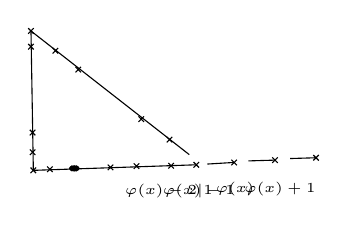
\begin{tikzpicture}[x=1cm,y=1cm]\draw (.02,1.77)--(.05,0)--(2.10,.07);\draw (.02,1.77)--(2.03,.20);\draw (2.26,.08)--(2.59,.10) (2.78,.12)--(3.12,.13) (3.31,.15)--(3.64,.16);
\foreach \x/\y in {.02/1.77,.02/1.57,.04/.48,.04/.23,.05/0,.26/.014,.57/.025,1.03/.037,1.36/.053,1.80/.058,2.12/.070,2.60/.10,3.12/.13,3.64/.16,.33/1.52,.62/1.28,1.42/.65,1.78/.39}{\draw (\x-.035,\y-.035)--(\x+.035,\y+.035) (\x-.035,\y+.035)--(\x+.035,\y-.035);}
\fill (.57,.025) ellipse (.07 and .04);
\node[below,font=\tiny] at (1.77,-.055) {$\varphi(x)-\unsure{2|1}$};\node[below,font=\tiny] at (2.15,-.055) {$\varphi(x)-1$};\node[below,font=\tiny] at (2.61,-.03) {$\varphi(x)$};\node[below,font=\tiny] at (3.18,-.03) {$\varphi(x)+1$};\end{tikzpicture}}

% L17–20, conclusion
La suite spectrale donne alors $H^{\unsure{n|*}}(X,g_*(G))\simeq H^n(x,G)$ pour $n\geq\varphi(x)+1$. Or, par l'hyp. a), le deuxième membre est nul, OK.
\scanpage{69}
% archive sheet number: 68

% L1–3, NB
\uline{NB} Si $f:X\to Y$ morphisme de type fini de schémas \unsure{loc|loc.} noeth, alors, avec la fonction $\unsure{\varphi|\phi}$ précédente, on a pour $x\in X$, $y=f(x)$

% L4, field inequality
\[ \varphi(x)\leq\varphi(y)+2\,\deg\mathrm{tr}\,k(x)/k(y) \]

% L5, crossed beginning
\deleted{Si \unsure{fonct.|pour|fonction} $\varphi$}
